\chapter{Relative Efficiency of Decoupled Flow Solver}
\label{chapter-eight}

At this point, the reacting gas adjoint in FUN3D has been utilized to obtain
sensitivity information needed to drive design optimization, and the
sensitivities of the fully coupled scheme have been validated against complex
frechet derivatives for accuracy.  A key point of this study is to demonstrate
the increase computational efficiency and relative memory saving of using a
decoupled variable set for the flow and adjoint solvers, instead of a fully
coupled variable set.  This chapter details the benefits of applying the
decoupled flow solver over the fully coupled solver for a variety of test cases,
including the annular jet demonstration problem.

\section{5 km/s Flow over Cylinder}
\label{sec:5-kps-cylinder}

Demonstrating the improved efficiency in cost and memory required to utilize the
decoupled scheme, and that both the fully coupled and decoupled approaches
converge to the same result, a grid convergence study was conducted on a simple
cylinder geometry (radius 0.5 m).  Due to the presence of strong shocks in blunt
body flows, it was advantageous to generate structured-type grids to preserve
grid alignment with the bow shock. A 50$\times$50, 100$\times$100, and
200$\times$200 family of grids were adapted using the adaptation capability in
FUN3D\cite{adaptation} to produce shock-aligned grids. These grids serve as a
surrogate for conducting a grid convergence study, in that differences observed
between the decoupled and fully coupled schemes decrease as the average mesh
spacing decreases.  These grids are unstructured, consisting totally of
hexahedra elements with a single cell in the spanwise direction, and the
50$\times$50 grid is shown in Figure \ref{grid}.  The cell elements of these
grids were also subdivided into tetrahedral elements, and it was verified that
there are no issues with a true unstructured grid topology.  The free stream
conditions used were $V_{\infty} = 5000\ m/s$, $\rho_{\infty}=0.001\ kg/m^3$,
and $T_\infty = 200\ K$.  Several chemical kinetics models were used, including
a 5-species model with 5 reactions, an 11-species model with 22 reactions, and
an 18-species model with 29 reactions.  All cases were run in thermodynamic
equilibrium, with a one-temperature model.

%------------------------------------------------------------------------------%
\begin{figure}[h]
	\centering
  \adjincludegraphics[width=0.8\textwidth,trim={0 4cm 0 4cm},clip]{figures/scitech/grid}
	\caption{50$\times$50 cylinder grid.}
  \label{grid}
\end{figure}
%------------------------------------------------------------------------------%

\subsection{Cylinder - Verification of Implementation}

In order to be valid, the decoupled scheme must yield converged solutions that
are nearly identical to those of the fully coupled system. To quantitatively
assess this, we compare the predicted surface pressure, surface temperature, and
the species composition on the stagnation line for both schemes.  Figure
\ref{pq} shows the predicted quantities on the 100$\times$100 grid, for species
mixture of N, $\text{N}_2$, O, $\text{O}_2$, and NO with five reactions. All
results are indeed nearly identical, with temperature and pressure matching
discretely to eight digits and the species mass fractions on the stagnation line
matching to four digits.  This difference was further reduced on the finest grid
level of 200$\times$200, suggesting that both schemes converge to the same
solution with grid refinement.
%------------------------------------------------------------------------------%
\begin{figure}[h!]
  \captionsetup[subfigure]{position=b}
  \centering
  \subcaptionbox{Surface pressure}{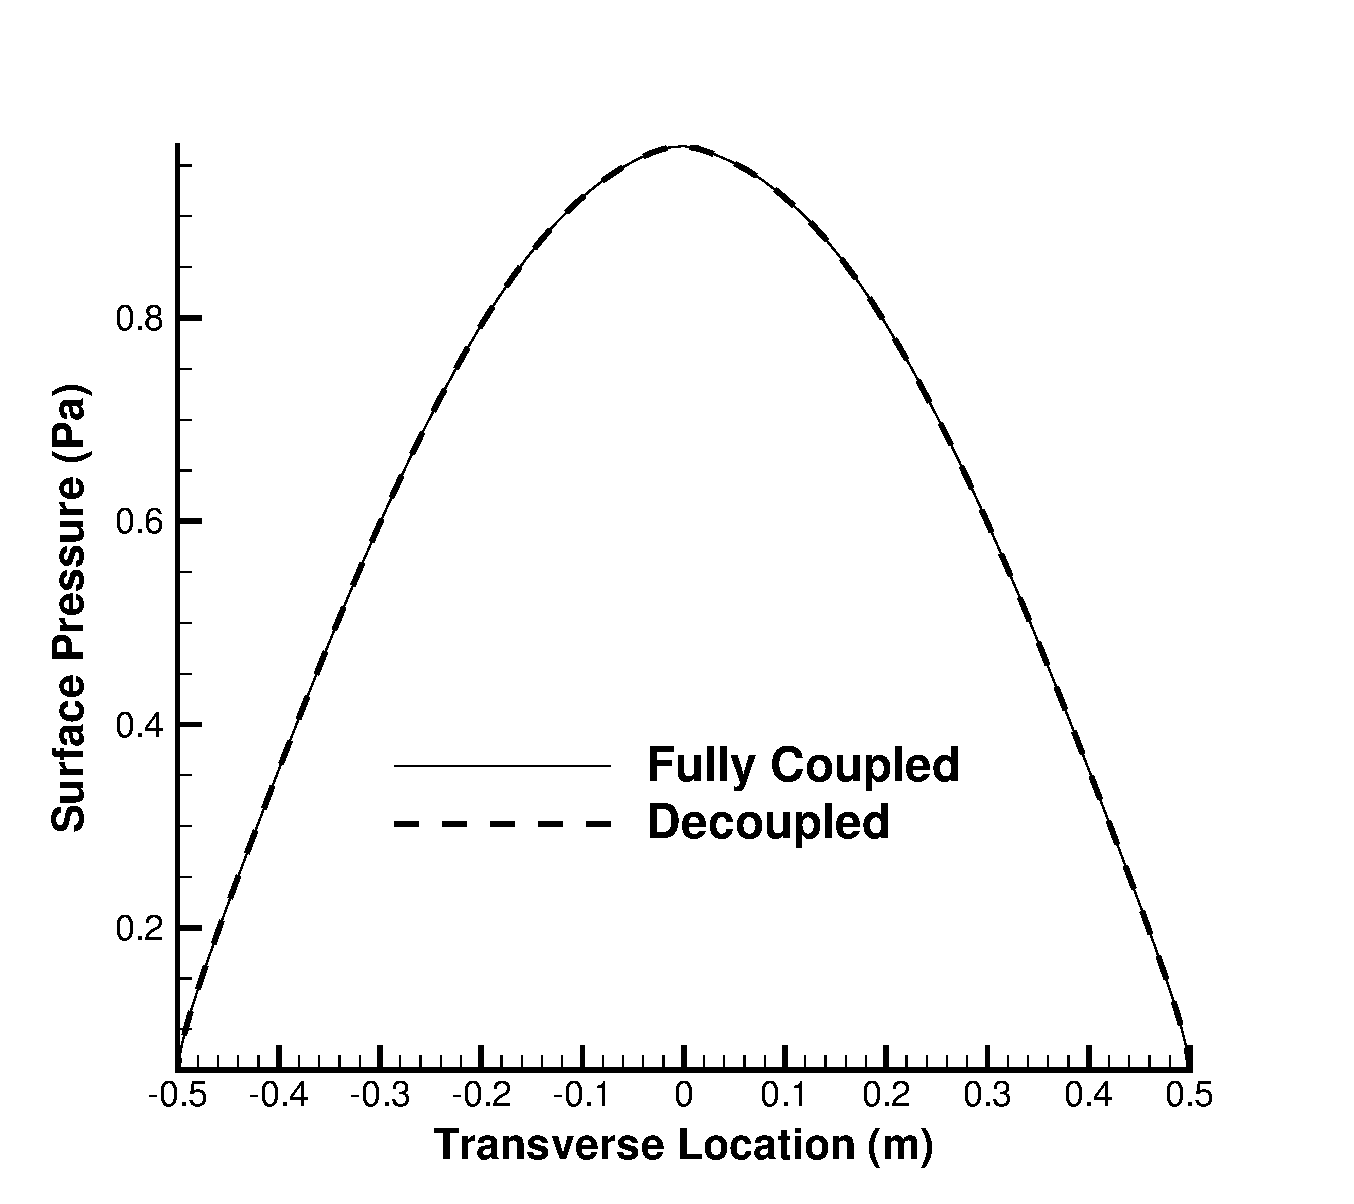
\includegraphics[width=0.3\linewidth]{figures/scitech/surface_pressure}}
  \subcaptionbox{Surface temperature}{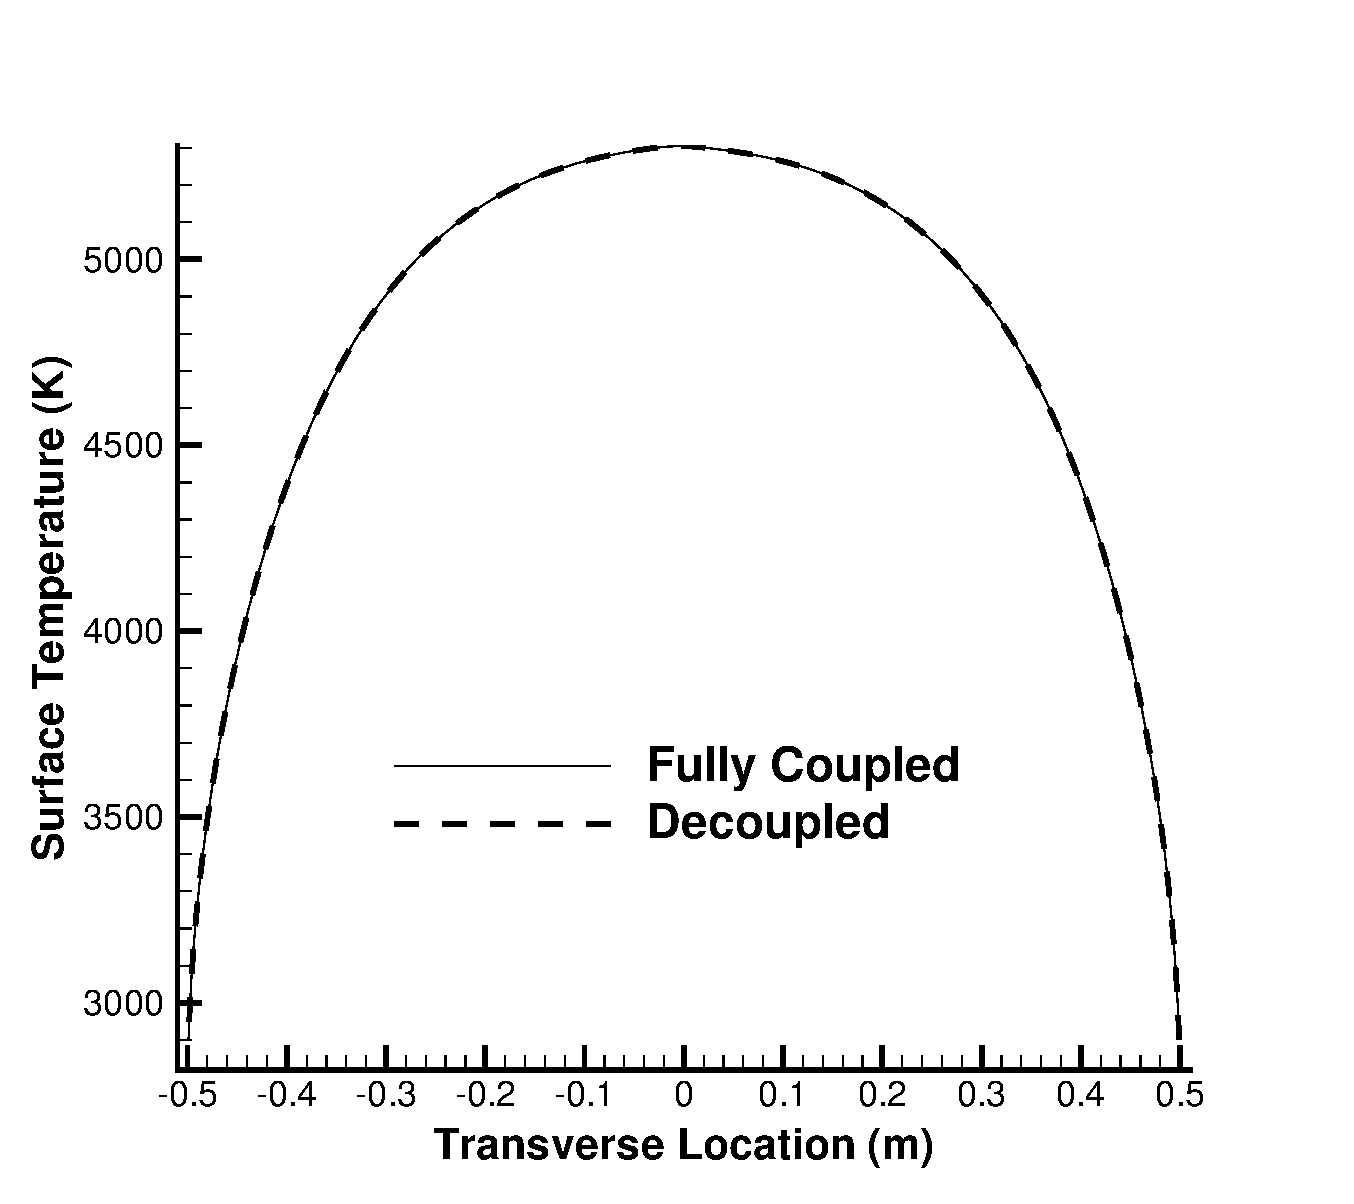
\includegraphics[width=0.3\linewidth]{figures/scitech/surface_temperature}}
  \subcaptionbox{Mass fractions on stagnation line}{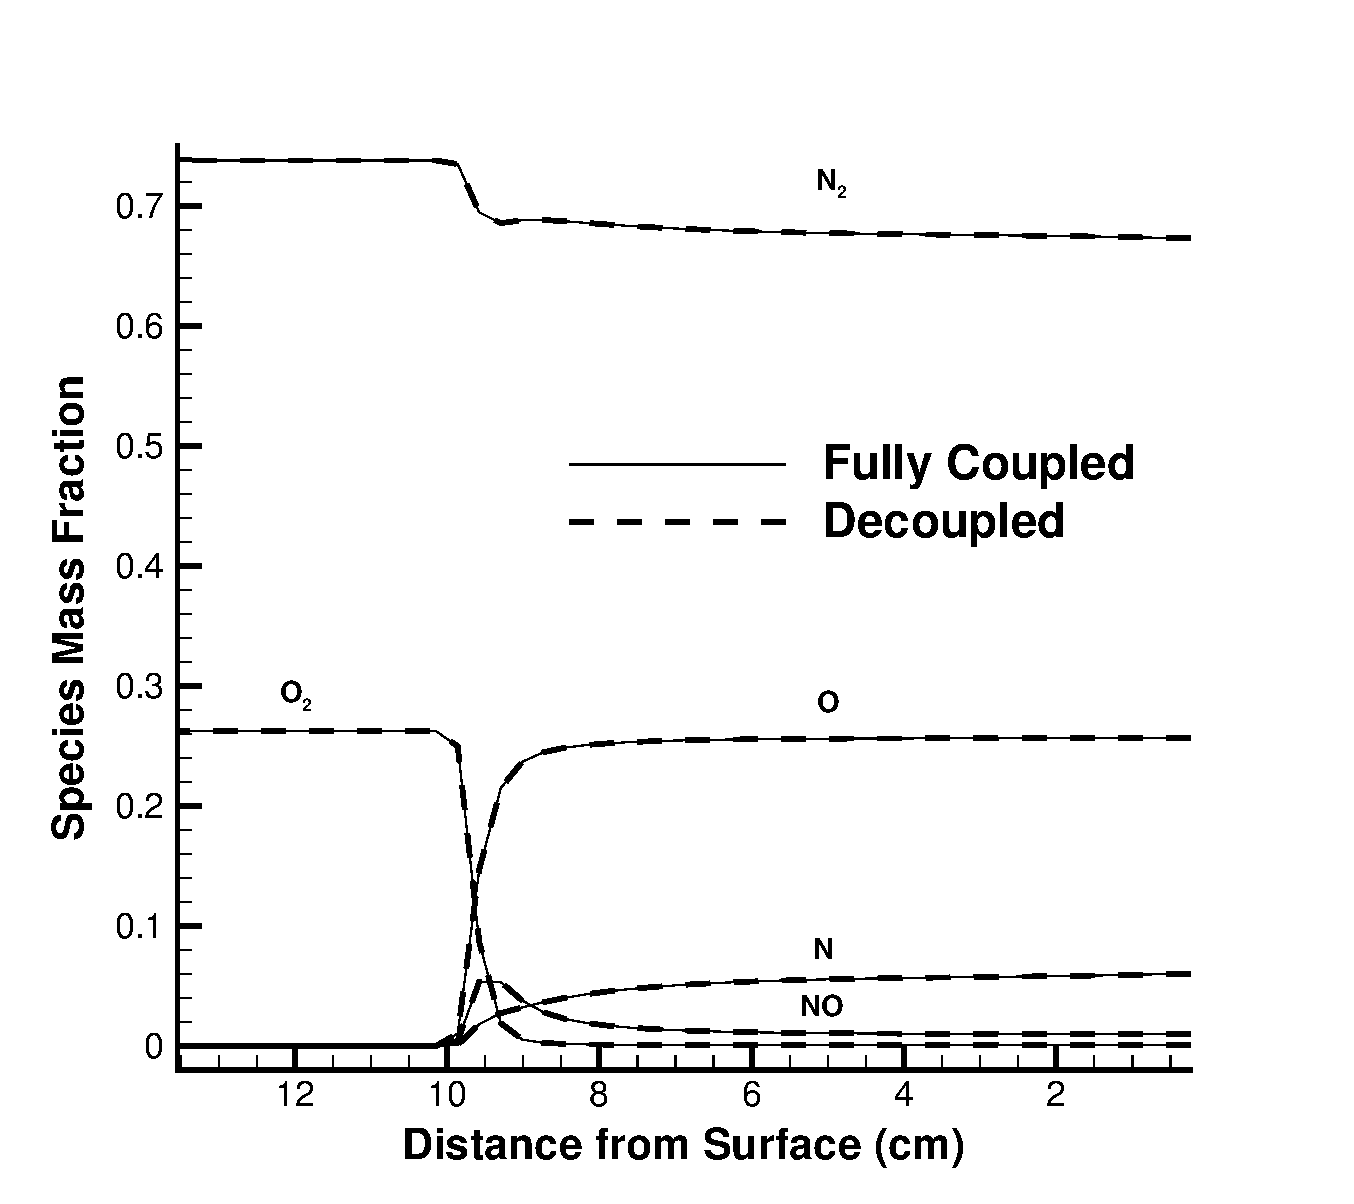
\includegraphics[width=0.32\linewidth]{figures/scitech/stag_line_mf}}
	\caption{Cylinder predicted quantities.}
	\label{pq}
\end{figure}
%------------------------------------------------------------------------------%

\subsection{Cylinder - Memory Cost}

In order to determine the required memory of the decoupled scheme compared
to the fully coupled scheme, a convergence study was conducted using
Valgrind\cite{valgrind} to determine the memory actually allocated by FUN3D for
an increasing number of species.  
Figure \ref{mem_req} shows that the relative memory cost converges asymptotically to
$\sim$1/4, which is nearly twice the predicted value of 1/7.  For the
implementation of FUN3D, this is correct because the off-diagonal entries are
reduced from double to single precision.  Each structured grid node has six
neighboring nodes, with the exception of those at the boundary.  Because each of
these six neighboring nodes yields single precision, off-diagonal Jacobian
elements, 
%------------------------------------------------------------------------------%
\begin{equation} 
  N_{nz} = \frac{6N_{nodes}}{2} = 3N_{nodes}
  \label{f3d_off_diag} 
\end{equation} 
%------------------------------------------------------------------------------%
Substituting \eref{f3d_off_diag} into \eref{mem_req_eq}, the relative memory
cost is:
%------------------------------------------------------------------------------%
\begin{equation} 
  Relative\ Memory\ Cost = 
  \frac{N_{nodes}}{N_{nodes} + N_{nz}} =
  \frac{N_{nodes}}{N_{nodes} + (3N_{nodes})}=\frac{1}{4}
\end{equation}
%------------------------------------------------------------------------------%
%------------------------------------------------------------------------------%
\begin{figure}[h] 
  \begin{center} 
    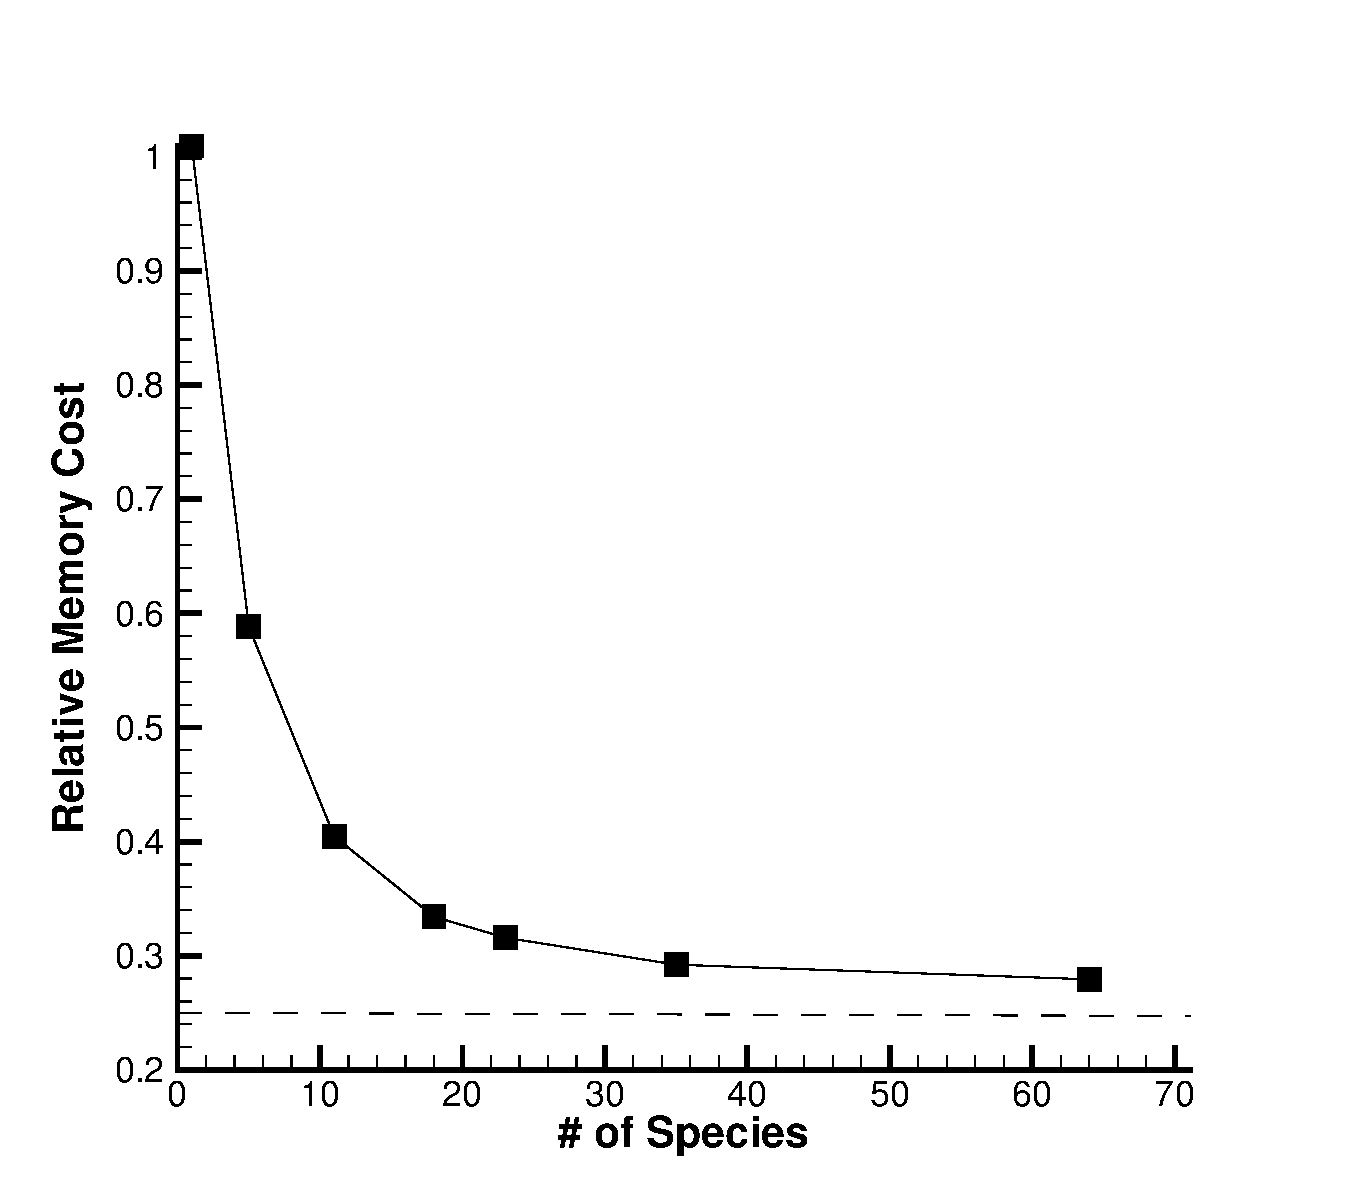
\includegraphics[width=0.45\textwidth]{figures/scitech/mem_req}
    \caption{Memory required convergence study} 
    \vspace{-2em}
    \label{mem_req}
    \end{center} 
\end{figure}
%------------------------------------------------------------------------------%
thus, the relative memory saved by using the decoupled scheme correctly
approaches a factor of 1/4.

\subsection{Cylinder - Computational Cost}

As stated before, the cost of solving the decoupled implicit system should scale
approximately linearly with the number of species, whereas the fully coupled
problem should scale quadratically; thus, the speedup of the implicit solve
should be approximately linear when comparing the decoupled and fully coupled
approaches.  Figure \ref{rel_speedup} shows this to be true for the cylinder test
case, and that the total speedup of the problem is less than that of just
the linear solve.  It is to be expected that the overall gains are not as large
as those for the implicit solve, since there are many other factors that
scale with the number of species, especially calculating the species source term
and its linearization.

%------------------------------------------------------------------------------%
\begin{figure}[h]
  \centering
  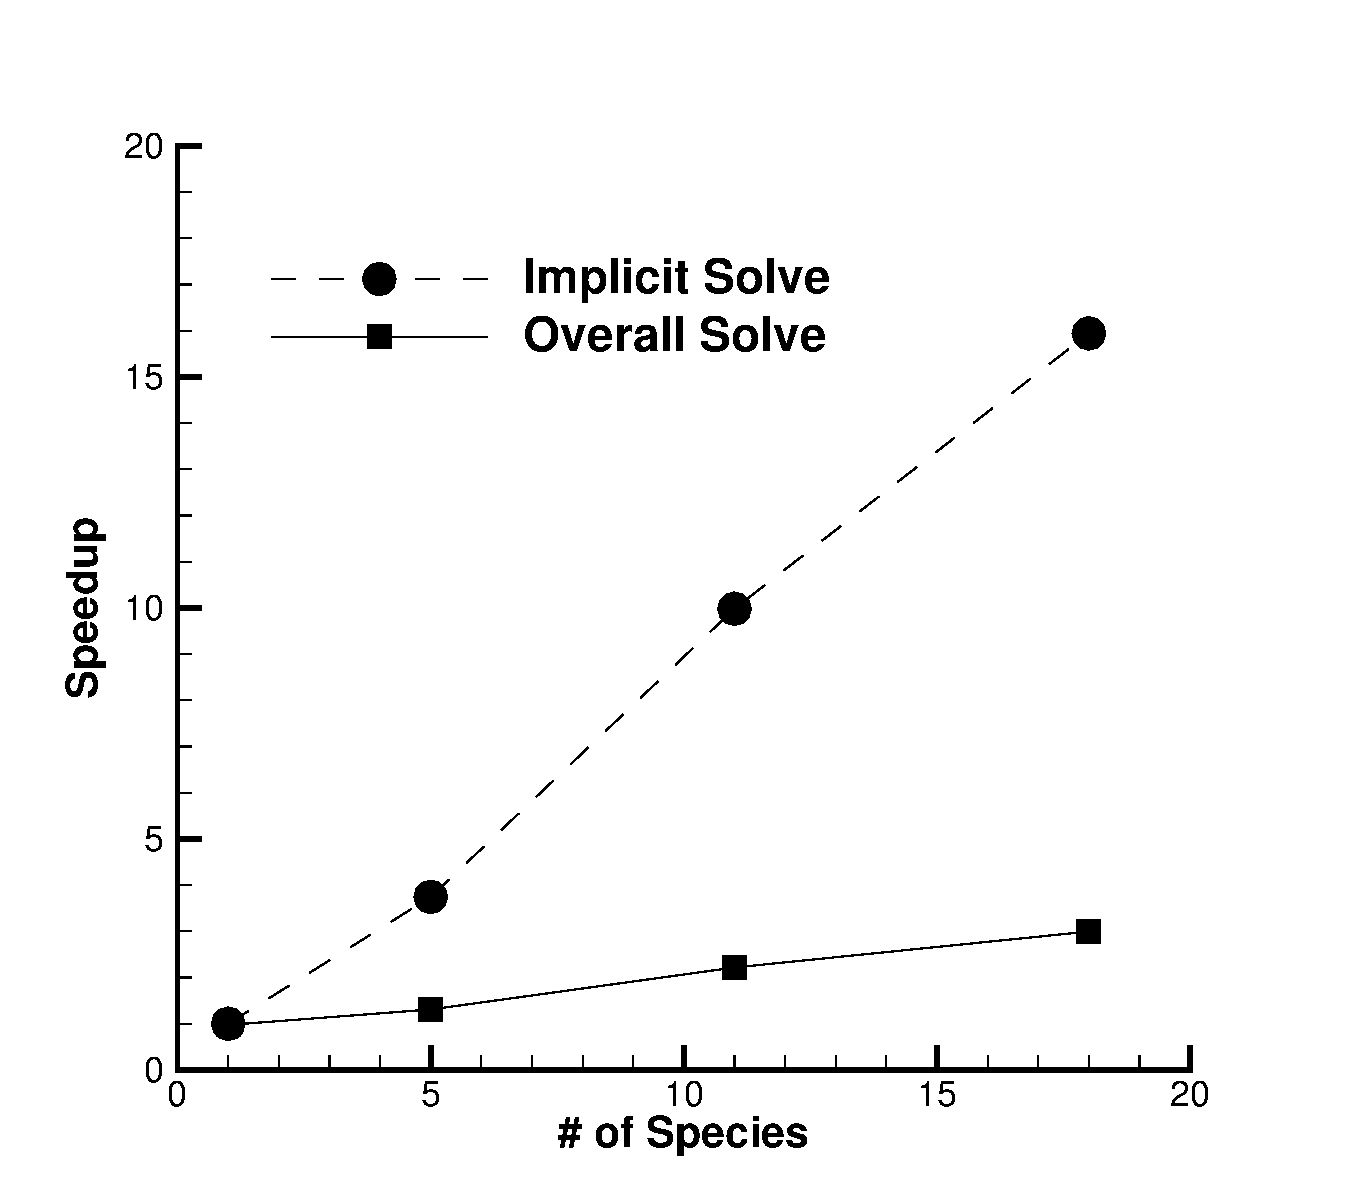
\includegraphics[width=0.45\textwidth]{figures/scitech/speedup} 
  \caption{ Relative speedup for the decoupled scheme vs. fully coupled scheme.}
  \label{rel_speedup} 
\end{figure}
%------------------------------------------------------------------------------%

\section{15 km/s Flow over Spherically-Capped Cone}
\label{sec:15-kps-sphere-cone}

To ensure that the decoupled scheme is robust and accurate at higher velocities, both the
fully coupled and decoupled approaches were run on a sphere-cone geometry
identical to that presented by Candler et. al. \cite{candler} (10 cm nose
radius, 1.1 m length, 8$^o$ cone angle).  For this case, a simple 64$\times$64
hexahedra grid was constructed, and freestream conditions were set as
$V_{\infty} = 15000\ m/s$, $\rho_{\infty}=0.001\ kg/m^3$, $T_\infty = 200\ K$.
It was discovered that CFL limitations for the decoupled scheme were
prohibitive, because of the stiffness of the chemical source term.  In order to
converge the scheme in a manner competitive with the fully coupled approach, it
was necessary to scale the magnitude of the source term contribution to the flux
balance by a value $\omega$, such that $0 \leq \omega \leq 1$.  To ensure that
the decoupled and fully coupled approaches yielded the same result, a ramping
scheme was implemented such that no scaling was performed on the source term
when the solution was in a converged state.

\subsection{Sphere-Cone - Verification of Implementation} 

As with the cylinder test case, the surface pressure and temperature were used
as metrics to determine that both the decoupled and fully coupled approaches
give the same answer when converged to steady-state. The species composition
consisted of N, $\text{N}_2$, O, $\text{O}_2$, NO, N$^+$, $\text{N}_2^+$, O$^+$,
$\text{O}_2^+$, NO$^+$, and electrons, with 22 possible reactions. Figure
\ref{cone_predictions} shows that both methods again yield similar results, and
the high stagnation temperature indicates that this is an inviscid,
one-temperature simulation.  This demonstrates that the decoupled approach is
able to converge to the same solution as the fully coupled solution, in spite of
the chemical reactions proceeding very rapidly due to a high stagnation
temperature.

%------------------------------------------------------------------------------%
\begin{figure}
	\centering
	\begin{subfigure}[b]{0.4\textwidth}
		\centering
		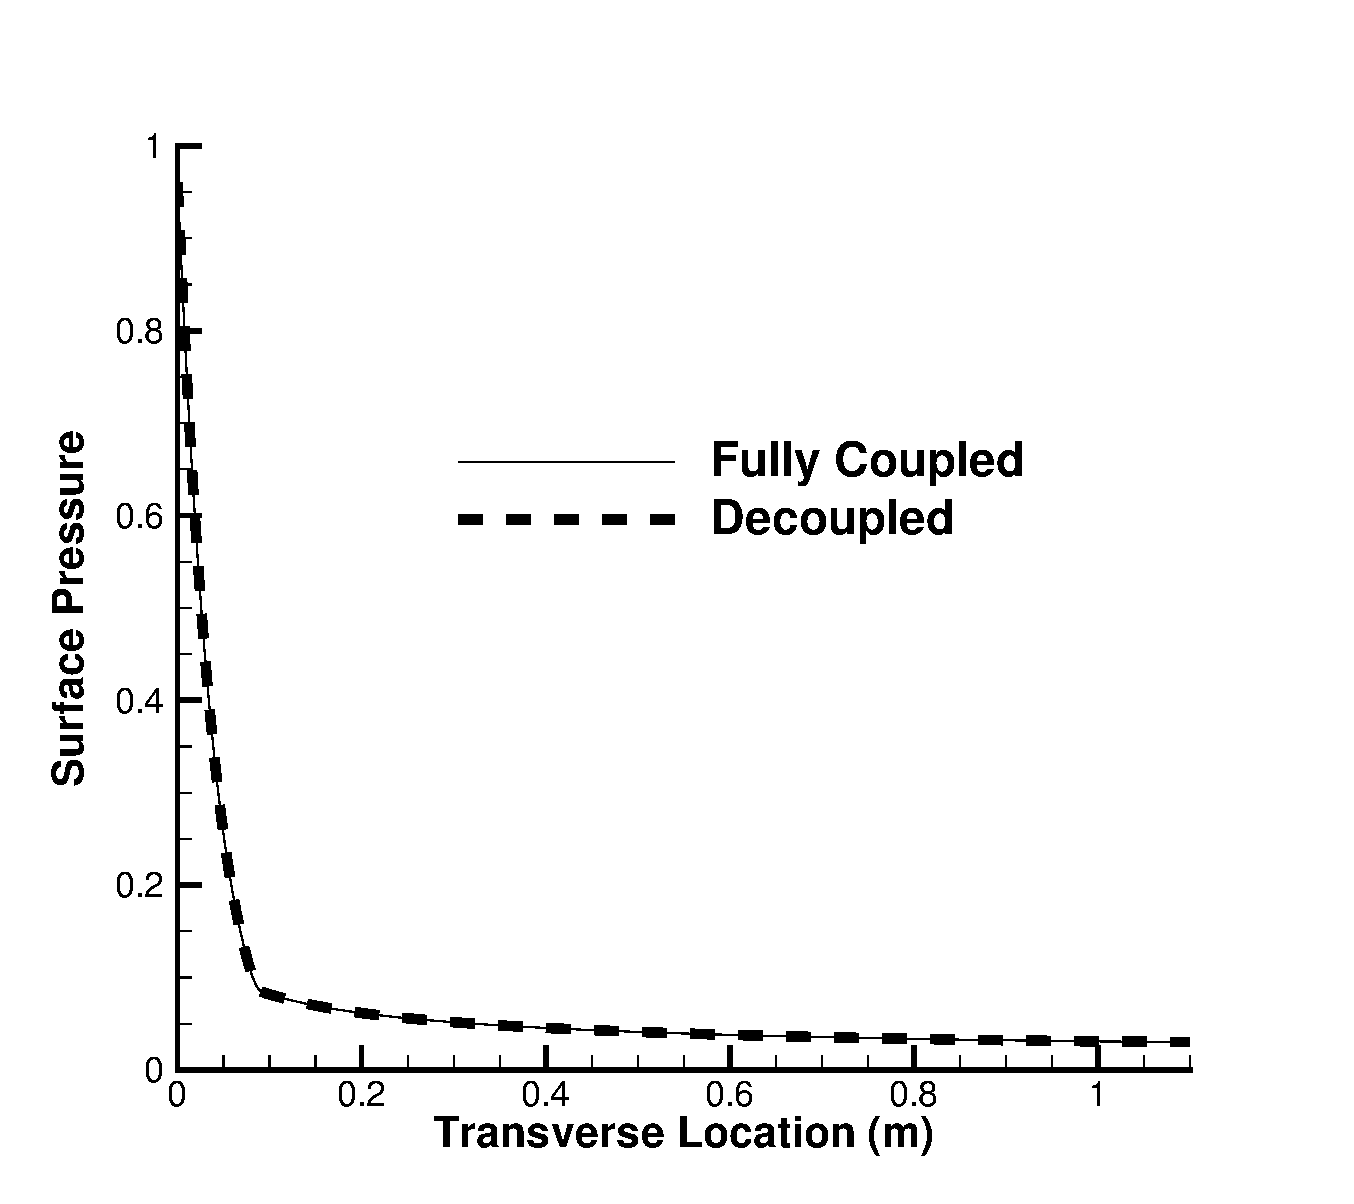
\includegraphics[width=\textwidth]{figures/scitech/surface_pressure_cone}
		\caption{Surface pressure}
		\label{cone_pressure}
	\end{subfigure}
	\begin{subfigure}[b]{0.4\textwidth}
		\centering
		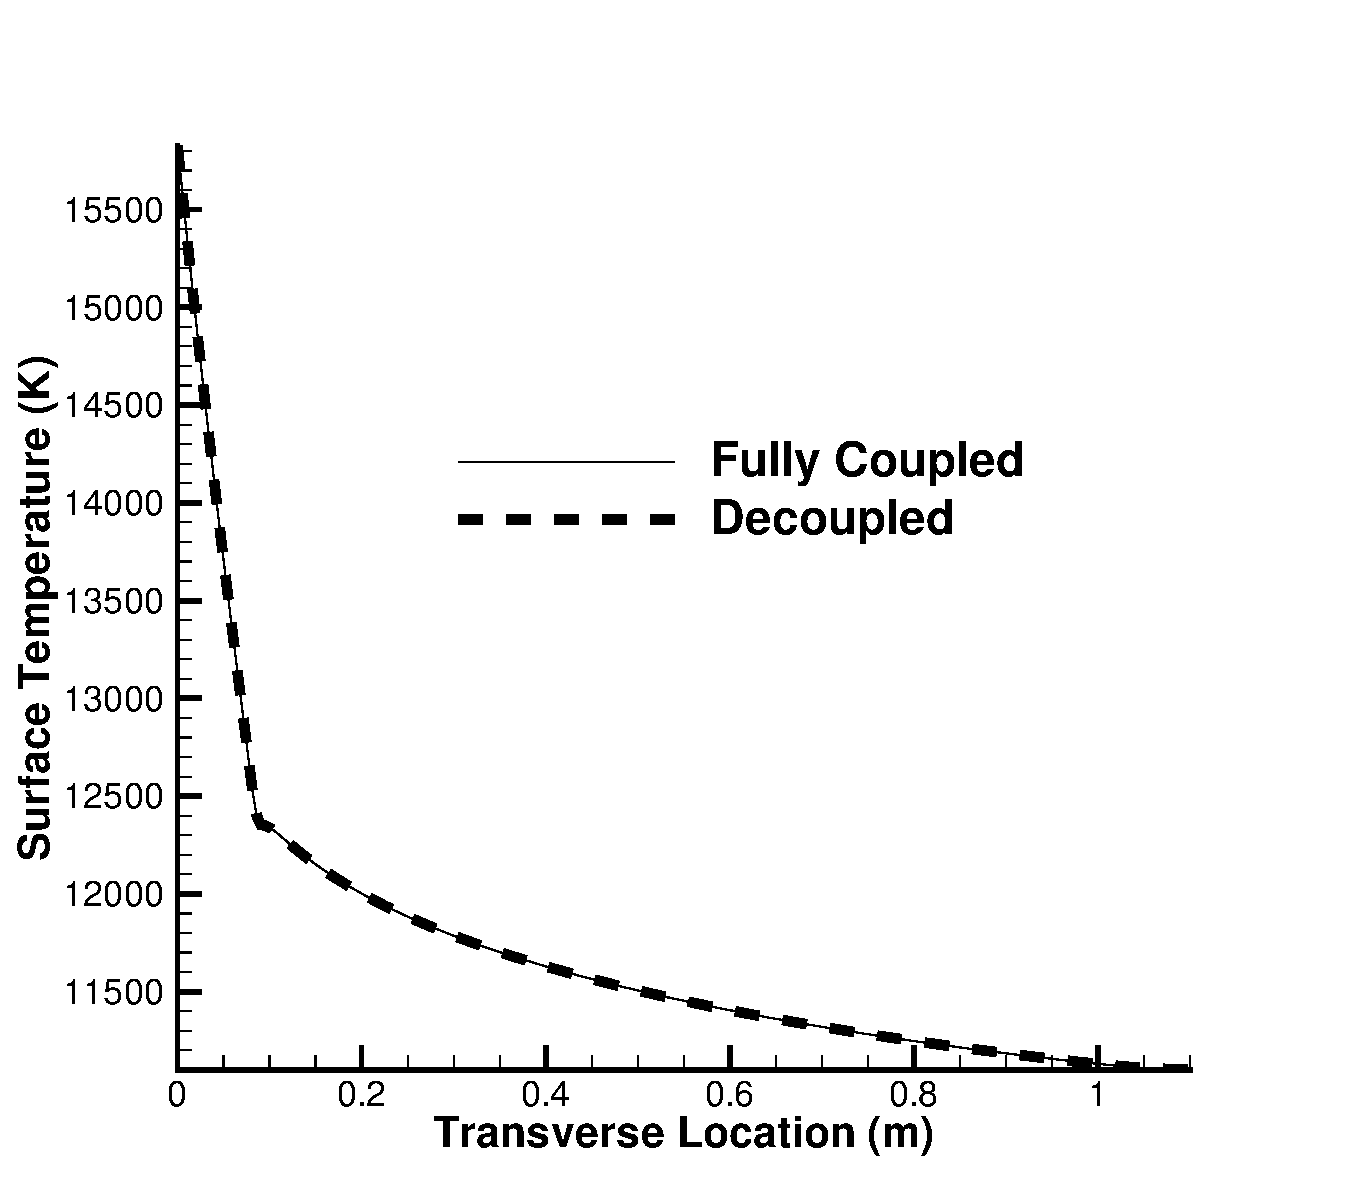
\includegraphics[width=\textwidth]{figures/scitech/surface_temperature_cone}
		\caption{Surface temperature}
		\label{cone_temp}
	\end{subfigure}
  \caption{ Sphere-cone predicted quantities. }
  \label{cone_predictions}
\end{figure}
%------------------------------------------------------------------------------%

\subsection{Sphere-Cone - Convergence Quality}

The limits on the stability of the decoupled scheme derives from introducing
explicitness in creating and destroying species.  By scaling the magnitude of
the chemical source term during the transient phase of the solve, this
instability can be mitigated, and the convergence of decoupled scheme approaches
that of the fully coupled scheme. Scaling of chemical source term was done
identically between the decoupled and fully coupled scheme by ramping the
factor $\omega$ from 0.001 to 1.0 over the first 500 timesteps. Figure
\ref{cone_convergence} shows that the convergence of both schemes progresses
nearly identically, with the decoupled scheme converging in significantly less
computational time and, interestingly, fewer timesteps.
%------------------------------------------------------------------------------%
\begin{figure}
	\centering
	\begin{subfigure}[b]{0.45\textwidth}
		\centering
    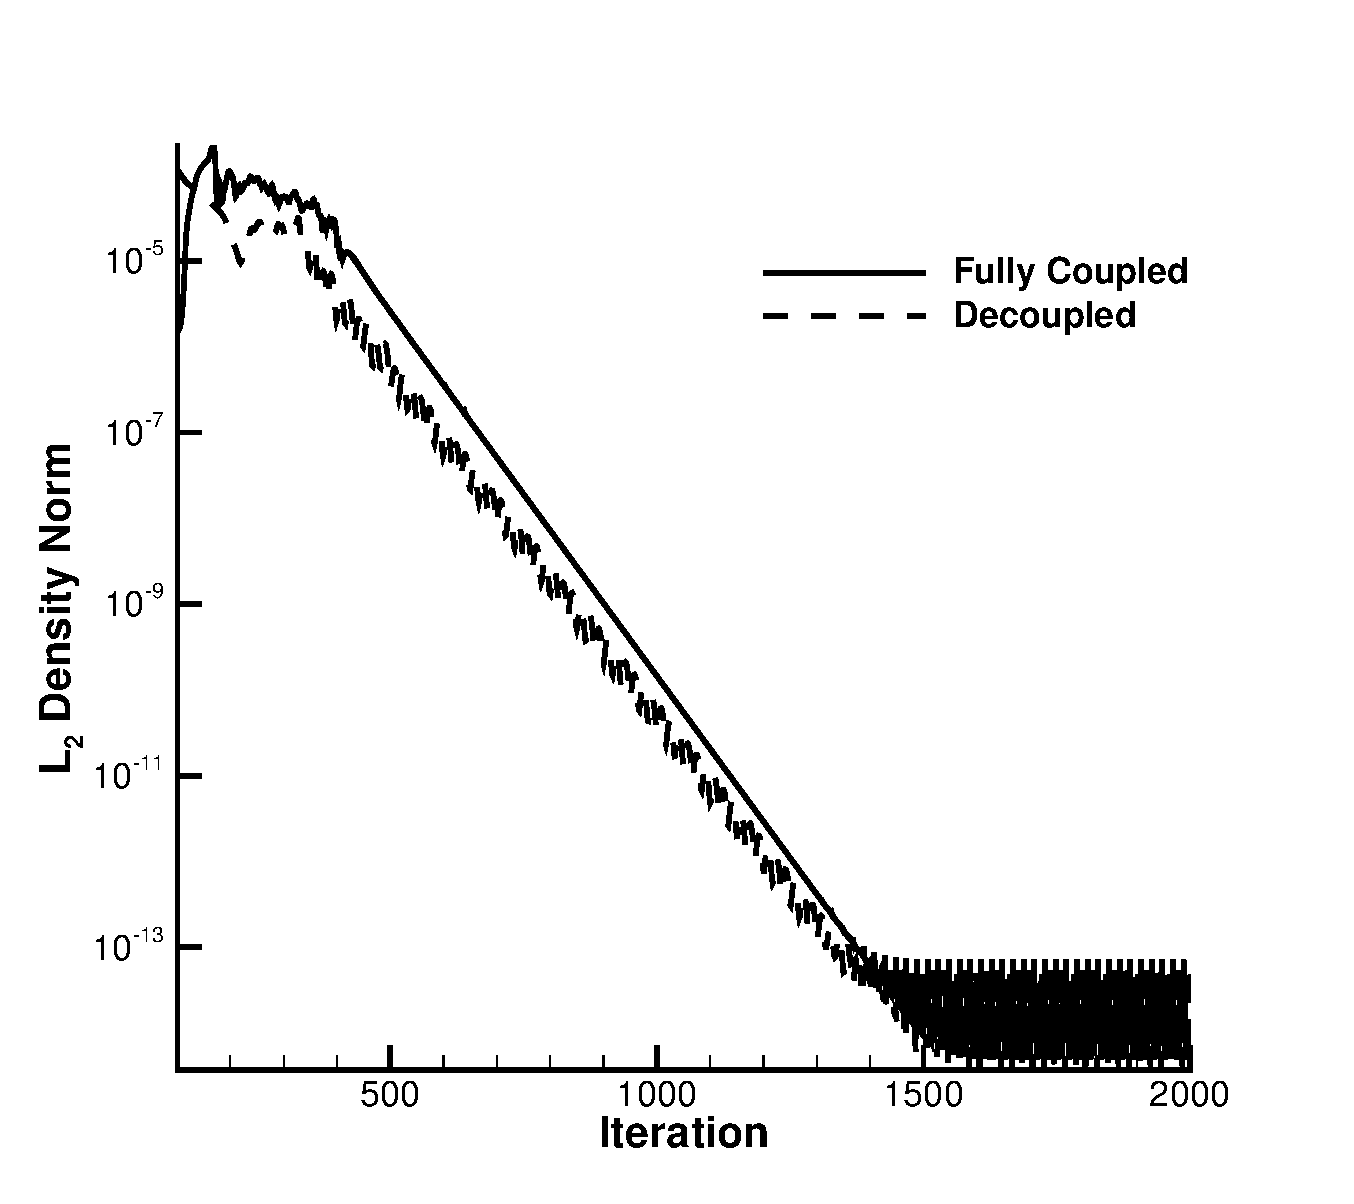
\includegraphics[width=\textwidth]{figures/scitech/cone_iteration}
		\caption{Iterations to convergence}
		\label{cone_iterations}
	\end{subfigure}
	\begin{subfigure}[b]{0.45\textwidth}
		\centering
		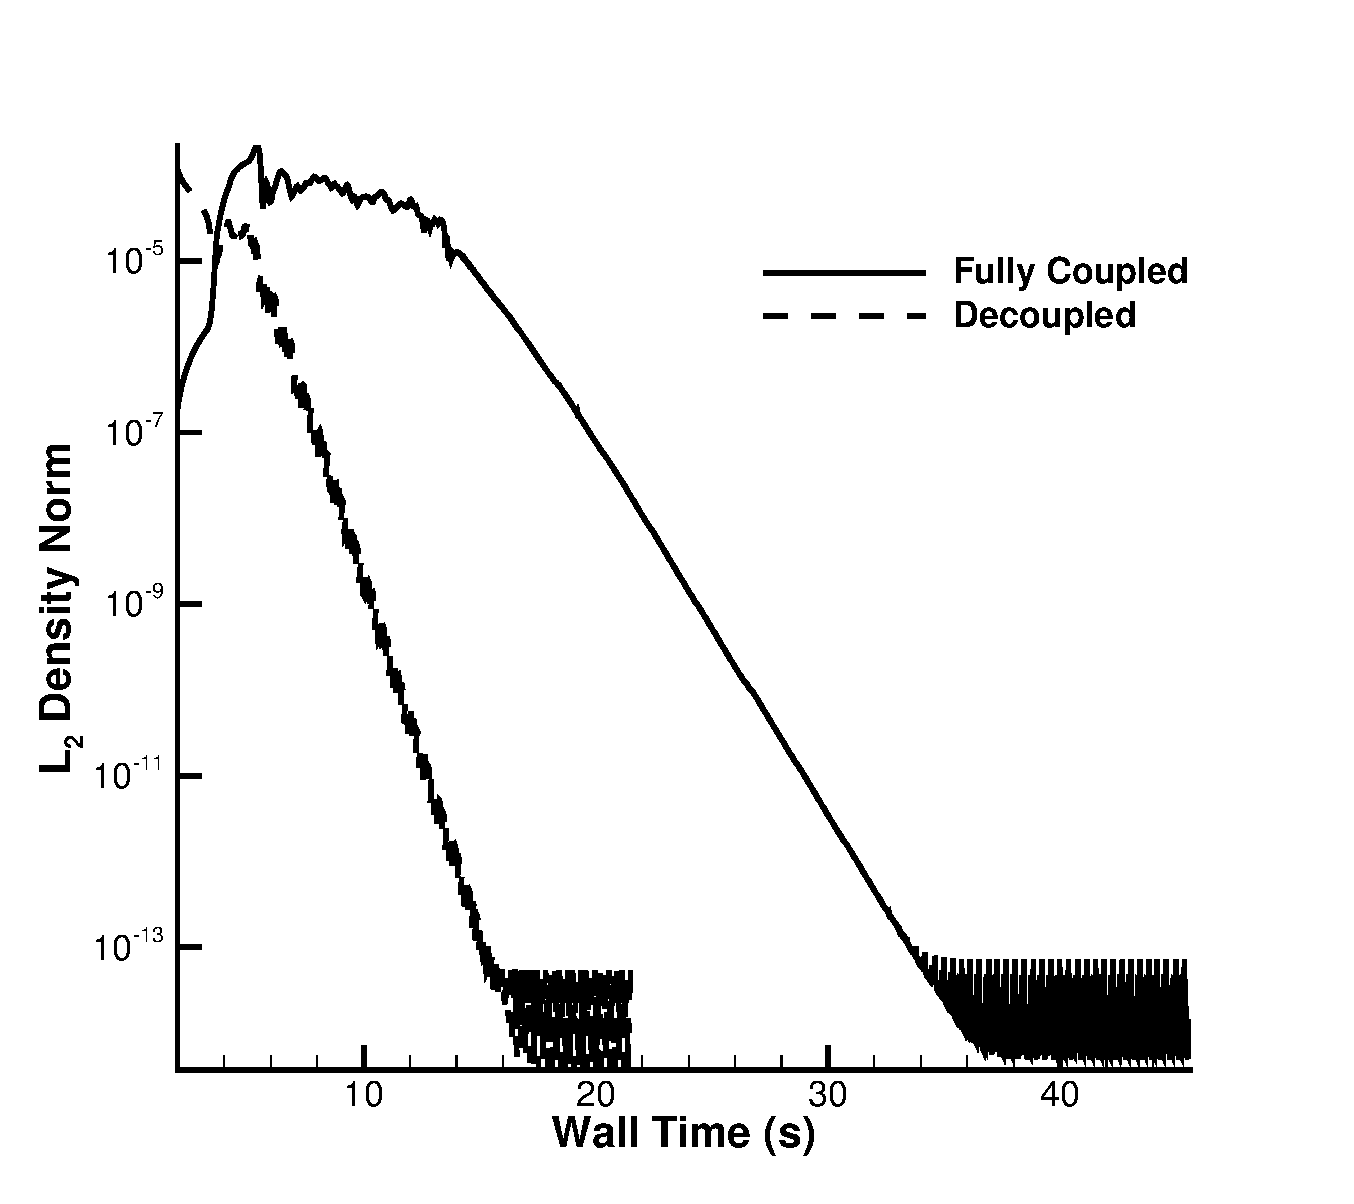
\includegraphics[width=\textwidth]{figures/scitech/cone_walltime}
    \caption{Computational time to convergence}
		\label{cone_walltime}
	\end{subfigure}
  \caption{ Sphere-cone convergence details. }
  \label{cone_convergence}
\end{figure}
%------------------------------------------------------------------------------%
This demonstrates that the decoupled scheme has significant potential to
improve the efficiency of high-velocity simulations, and that the stiffness of
the source term can be overcome in the presence of large chemical reaction
rates.



\subsection{Sphere Cone - Convergence Improvement with Exact First-Order Linearizations}

An important benefit of implementing an adjoint solver in FUN3D comes the
requirement of exact linearizations, because the linearizations needed to form
the residual in the adjoint solver can be reused by the flow solver.
Due to the high storage requirements associated with exactly linearizing the
gradient terms in the reconstruction, an approximate jacobian is used in the
flow solver.  This approximate jacobian consists of linearizations of the
first-order scheme, as is used to solve the governing equations via defect
correction.  Previously, the reacting gas path employed a jacobian also, that
approximated the linearizations of the Roe FDS scheme\cite{gnoffo-tp} as
%------------------------------------------------------------------------------%
\begin{equation}
  \rdiff{}{\mU} = 
  \frac{1}{2} \left( \rdiff{c}{\mU} + \rdiff{\tilde{c}}{\mU} \right)
  \label{approx-roe-jac}
\end{equation}
%------------------------------------------------------------------------------%
where $\rdiff{c}{\mU}$ is the linearization of the convective portion of the Roe
FDS scheme, and $\rdiff{\tilde{c}}{\mU}$ is the approximation to the dissipation
term in the Roe RDS scheme, formed by evaluating $\rdiff{c}{\mU}$ with Roe
averaged quantities.  This approximation has been is used by others
\cite{rinaldi2014exact} to mitigate the development time of implementing an
exact linearization of the dissipation term in the Roe FDS scheme, as well the
large computational cost in computing those linearizations at each jacobian
update.

To demonstrate any benefit of the exact linearization of the Roe FDS scheme on
iterative convergence of the flow solver, the sphere cone case was converged
using both the jacobian employing exact linearizations of the Roe FDS scheme
flux, and the jacobian employing the approximation in \eref{approx-roe-jac}.
%------------------------------------------------------------------------------%
\begin{figure}[h]
  \centering
  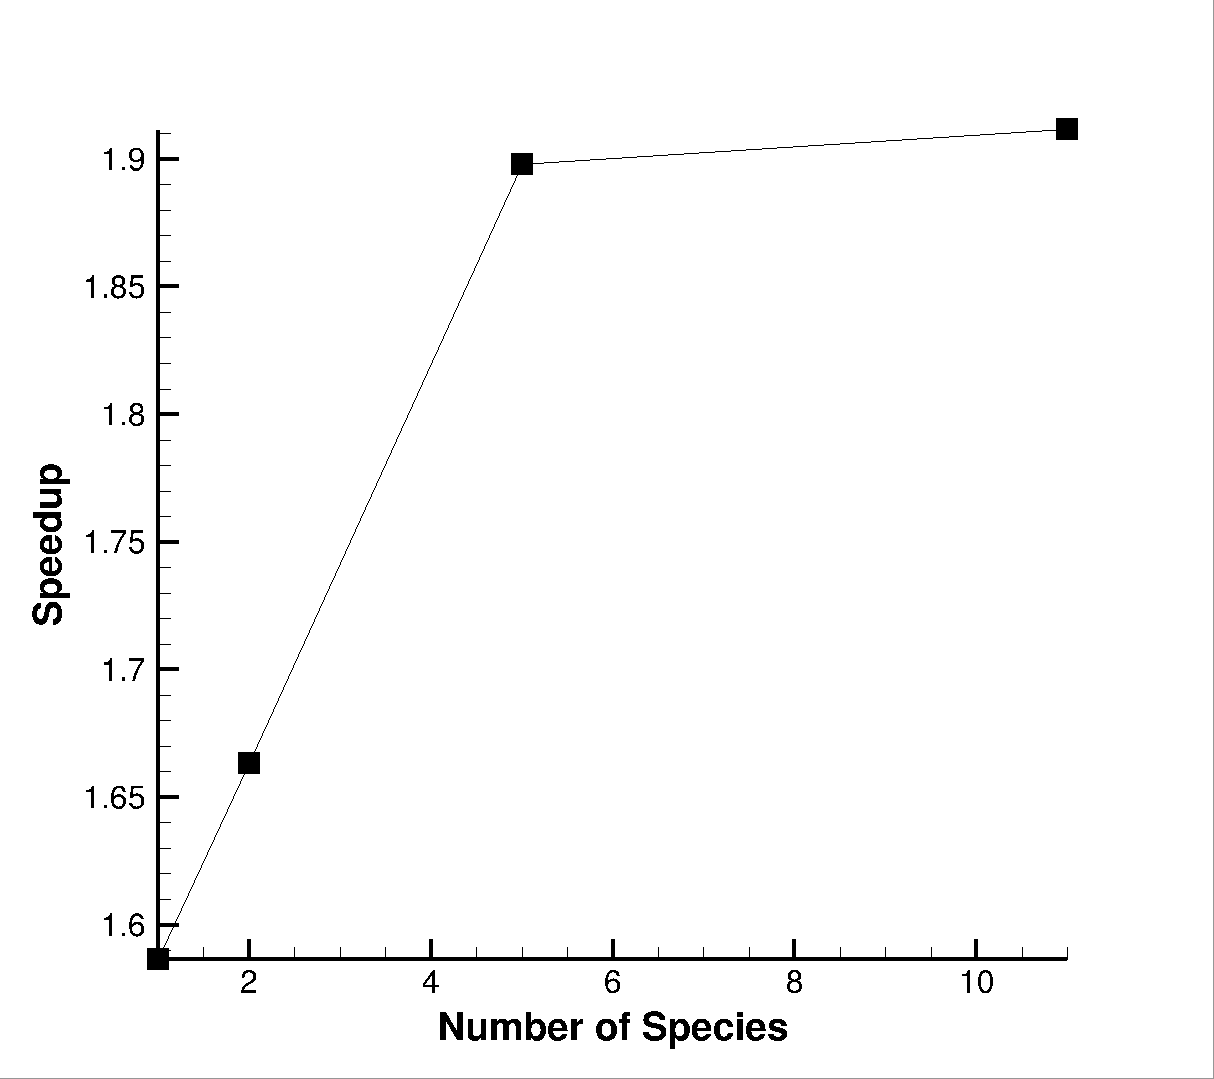
\includegraphics[width=0.5\textwidth]{figures/flow-efficiency/exact-approx-speedup.png}
  \caption{Relative Speedup Using Exact Linearizations}
  \label{fig:exact-approx-speedup}
\end{figure}
%------------------------------------------------------------------------------%
\fref{fig:exact-approx-speedup} shows that up to a five-species air mixture, the
convergence to steady state is completed in $58\%$ to $90\%$ less simulation
time.  For the 11 species air mixture, involving ionization, the speed up
promptly plateaus, as the additional costs incurred by computing the exact
linearizations supercede the improved iterative convergence.  It can be inferred
from \fref{fig:exact-approx-speedup} that the improvements compounded by the
decoupled scheme, which affords iterative converge similar to the exact fully
coupled scheme, will be significantly faster than the baseline scheme that was
originally implemented in the reacting gas path of FUN3D.

\section{Re-entry Vehicle with Retro-Firing Annular Jet}

The demonstration problem presented in \crefs{chapter-five}{chapter-six}
presents the most challenging problem for the decoupled scheme, due to the
Hydrogen-air combustion.  To verify that the solution is not effected by
employing the decoupled scheme over the fully coupled scheme, the comparison is
made between solutions of the decoupled and fully coupled flow solvers on the
cost function component quantities in \sref{cost-func-components}.  The
freestream conditions in \tref{tab:flow-conditions} were used for this
comparison, along with the plenum conditions in \tref{tab:plenum-conditions}.

\subsection{Annular Jet: Verification of Implementation}

Due to startup transients, where reaction rates grew very large as nearly all
$H_2$ and $O_2$, and most of $N_2$, dissociated near the stagnation region, the
source term scaling factor, $\omega$, was employed for this problem to maintain
stability.  It was empirically determined that the source term scaling could be
removed within the first third of the way to convergence for this problem.


